\begin{block}{Répartition des macro-structures}
    L'auteur insère des annotations de groupes sur les éléments de la partition interactive : 
    
    \begin{figure}
        \begin{tikzpicture}[scale=4]
        \input{scores/general.tex}
        \end{tikzpicture}
        \caption{Les annotations $G_{1..5}$ s'appliquent récursivement sur les contenus}
    \end{figure}

    On introduit trois modes d'exécution s'appliquant à un niveau hiérarchique donné~:
	\begin{itemize}
		\item \textbf{Exécution indépendante}~: chaque client du groupe exécute le scénario à son rythme ; les clients des autres groupes ne l'exécutent pas.
		\item \textbf{Partage complet}~: tous les clients partagent la même ligne temporelle récursivement ; chacune exécute les contenus propres à son groupe (fig.~\ref{fig.reparti}).
		\item \textbf{Partage mixte}~: certaines branches peuvent être exécutées par certains clients et pas par d'autres ; des resynchronisations peuvent avoir lieu en des points donnés par le compositeur.
	\end{itemize}
    
    \begin{figure} 
        \centering
        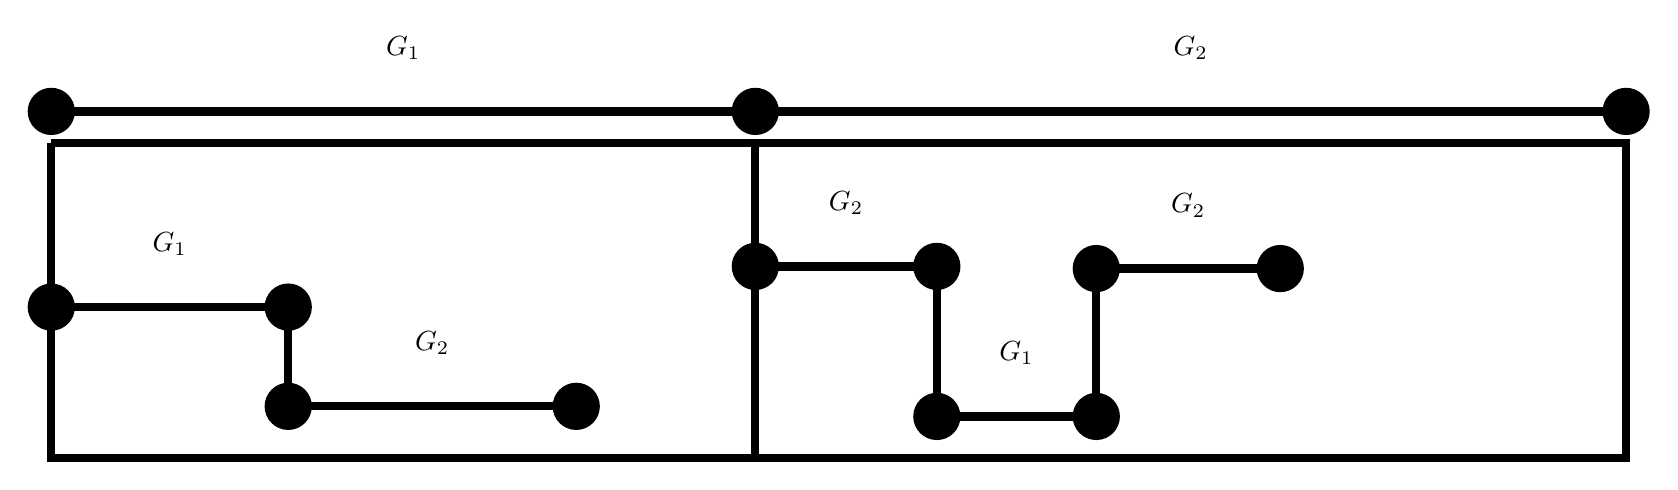
\begin{tikzpicture}[scale=4]
            \fill (0, 2.20767) circle (0.075) ; % State.1 
\fill (2.23529, 2.20767) circle (0.075) ; % State.2 
\fill (5, 2.20767) circle (0.075) ; % State.3 
\draw[line width=3pt] (0, 2.23364)  -- (0, 2.20767) ; % TimeNode.0 
\draw[line width=3pt] (2.23529, 2.20767)  -- (2.23529, 2.20767) ; % nook18bout42 
\draw[line width=3pt] (5, 2.20767)  -- (5, 2.20767) ; % nato89loop85 
\draw[line width=3pt] (0, 2.20767)  -- (2.23529, 2.20767) ; % step8duct27 
\draw (1.11765, 2.40767) node {$G_1$}; % step8duct27 
\draw[line width=3pt] (0, 2.10767)  -- (2.23529, 2.10767)  -- (2.23529, 1.10767)  -- (0, 1.10767)  -- (0, 2.10767) ;
\draw[line width=3pt] (2.23529, 2.20767)  -- (5, 2.20767) ; % what68step1 
\draw (3.61765, 2.40767) node {$G_2$}; % what68step1 
\draw[line width=3pt] (2.23529, 2.10767)  -- (5, 2.10767)  -- (5, 1.10767)  -- (2.23529, 1.10767)  -- (2.23529, 2.10767) ;



\fill (0, 9.28641 - 7.7) circle (0.075) ; % State.1 
\fill (2.25694 / 3, 9.28641 - 7.7) circle (0.075) ; % State.2 
\fill (2.25694 / 3, 8.97129 - 7.7) circle (0.075) ; % State.3 
\fill (5 / 3, 8.97129 - 7.7) circle (0.075) ; % State.4 
\draw[line width=3pt] (2.25694 / 3, 9.28641 - 7.7)  -- (2.25694 / 3, 8.97129 - 7.7) ; % loge35long20 
\draw[line width=3pt] (5 / 3, 8.97129 - 7.7)  -- (5 / 3, 8.97129 - 7.7) ; % wire36tick25 
\draw[line width=3pt] (0, 9.28641 - 7.7)  -- (2.25694 / 3, 9.28641 - 7.7) ; % sack65taft69 
\draw (1.12847 / 3, 9.48641 - 7.7) node {$G_1$}; % sack65taft69 
\draw[line width=3pt] (2.25694 / 3, 8.97129 - 7.7)  -- (5 / 3, 8.97129 - 7.7) ; % loon80rink81 
\draw (3.62847 / 3, 9.17129 - 7.7) node {$G_2$}; % loon80rink81 


\fill (2.23529 + 0, 9.56564 - 7.85) circle (0.075) ; % State.0 
\fill (2.23529 + 1.72897 / 3, 9.56564 - 7.85) circle (0.075) ; % State.1 
\fill (2.23529 + 1.72897 / 3, 9.08927 - 7.85) circle (0.075) ; % State.2 
\fill (2.23529 + 3.24766 / 3, 9.08927 - 7.85) circle (0.075) ; % State.3 
\fill (2.23529 + 3.24766 / 3, 9.55873 - 7.85) circle (0.075) ; % State.4 
\fill (2.23529 + 5 / 3, 9.55873 - 7.85) circle (0.075) ; % State.5 
\draw[line width=3pt] (2.23529 + 0, 9.56564 - 7.85)  -- (2.23529 + 0, 9.56564 - 7.85) ; % TimeNode.0 
\draw[line width=3pt] (2.23529 + 1.72897 / 3, 9.56564 - 7.85)  -- (2.23529 + 1.72897 / 3, 9.08927 - 7.85) ; % jogs95rang7 
\draw[line width=3pt] (2.23529 + 3.24766 / 3, 9.55873 - 7.85)  -- (2.23529 + 3.24766 / 3, 9.08927 - 7.85) ; % haul29dade96 
\draw[line width=3pt] (2.23529 + 5 / 3, 9.55873 - 7.85)  -- (2.23529 + 5 / 3, 9.55873 - 7.85) ; % vane42mets16 
\draw[line width=3pt] (2.23529 + 0, 9.56564 - 7.85)  -- (2.23529 + 1.72897 / 3, 9.56564 - 7.85) ; % scum85toss49 
\draw (2.23529 + 0.864486 / 3, 9.76564 - 7.85) node {$G_2$}; % scum85toss49 
\draw[line width=3pt] (2.23529 + 1.72897 / 3, 9.08927 - 7.85)  -- (2.23529 + 3.24766 / 3, 9.08927 - 7.85) ; % woof52dyad40 
\draw (2.23529 + 2.48832 / 3, 9.28927 - 7.85) node {$G_1$}; % woof52dyad40 
\draw[line width=3pt] (2.23529 + 3.24766 / 3, 9.55873 - 7.85)  -- (2.23529 + 5 / 3, 9.55873 - 7.85) ; % eben10crux7 
\draw (2.23529 + 4.12383 / 3, 9.75873 - 7.85) node {$G_2$}; % eben10crux7 


        \end{tikzpicture}
        \caption{Une exécution répartie hiérarchique n'est possible qu'en cas de partage complet~: sinon il est impossible d'assurer la cohérence entre machines.}
        \label{fig.reparti}
    \end{figure}
    
    \begin{figure}
        \includegraphics[scale=0.5]{images/quarre.jpg}
        \caption{Quarrè (Pierre Cochard, SCRIME, 2016) : une installation en son spatialisé avec plusieurs téléphones. La répartition est réalisée manuellement.}
    \end{figure}
\end{block}